\documentclass[a4paper,11pt,dvipdfmx]{ujarticle}
% パッケージ
\usepackage{graphicx}
\usepackage{url}
% レイアウト指定を記述したファイルの読み込み
%!TEX root = exercise.tex

\hoffset=-1in
\voffset=-0.5pt
\advance\textwidth2in
\advance\textheight1in
\topmargin=0pt
\headsep=0pt
\headheight=0pt


% タイトルと氏名を変更せよ.
\title{日本におけるデジタル化の状況}
\author{G585112025 海川 啄実}

\begin{document}

\maketitle %ここにタイトルが入る

\section{デジタル競争力ランキング}
    国際経営開発研究所(IMD)の調査\cite{imd}によると,日本のデジタル競争力のラン
キングは図\ref{fig:デジタル}に示すように,,調査対象の64ヵ国中,総合で28位,準備分野で27位
となっている.

\begin{figure}[htbt]
    \centering
    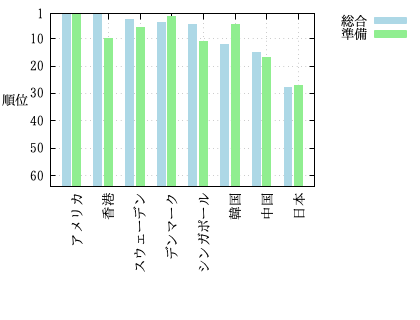
\includegraphics{表1.png}
    \caption{デジタル競争力ランキング(64ヵ国中)}\label{fig:デジタル}
\end{figure}

\newpage

\section{ブロードバンドの整備状況}

OECDによるブロードバンド回線の普及に関する調査\cite{oecd}によると,
表\ref{tbl:利用状況}に示すように,日本における100人当た
りの光ファイバー回線の加入者は29.0で,韓国,スウェーデン,ノルウェーに続
いて第4位になっている.

\begin{table}[htbp]
    \centering
    \caption{光ファイバー回線の加入者数(100人あたり)}
    \label{tbl:利用状況}

    \begin{tabular}{|c|l|r|}\hline
        順位 & 国名 & 加入者数 \\\hline
        1位 & 韓国 & 38.2 \\\hline
        2位 & スウェーデン & 31.9 \\\hline
        3位 & ノルウェー & 29.5 \\\hline
        4位 & 日本 & 29.0 \\\hline
        5位 & アイスランド & 28.8 \\\hline
        6位 & スペイン & 27.3 \\\hline
        7位 & ポルトガル & 25.1 \\\hline
        8位 & ニュージーランド & 23.6 \\\hline
        9位 & リトアニア & 22.3 \\\hline
        10位 & フランス & 21.2 \\\hline
    \end{tabular}
\caption{加入者数上位10カ国}
\end{table}

\section{考察}
\begin{itemize} 
   \item 日本はブロードバンドの整備において世界でも上位に位置しており、物理的なインフラ環境は非常に整っている。
 一方で、デジタル競争力ランキングでは中位にとどまっており、デジタル化の「質」や「活用」の面で課題があることを示している。
   \item デジタル競争力を構成する要素には、技術的な準備だけでなく、人材育成、組織の適応力、政策の柔軟性、データ活用の推進などが含まれる。
インフラの整備だけでは十分でなく、こうしたソフト面の改革が必要である。 
\end{itemize}

% ここから本文
% 節見出し: \section{}
% を使う

% 本文(1)
%  参考文献の参照: \cite{}
%  図番号の参照: \ref{}
% を使う
% 文献データベースのキーワードは oecd と imd
% になっている.

% 図の挿入
% \includegraphics{}
% を
% \begin{figure}[htbp]
% \end{figure}
% で囲み
% \caption{}
% で図のタイトルを入れる.
% \label{}
% を使って図番号が参照できるようにする
% また,
% \centering
% で図が中央に来るようにする

% ーーー
% 節見出し(2)

% 本文(2)

% 表の挿入
% \begin{tabular}
% \end{tabular}    
% による表の記述を 
% \begin{table}[htbp]
% \end{table}
% で囲み
% \caption{}
% で表のタイトルを入れる.
% \label{}
% を使って表番号が参照できるようにする
% また,
% \centering
% で表が中央に来るようにする

% ーーー
% 見出し(3)
% 考察
%
% \begin{itemize}
% \end{itemize}
% を使って箇条書きで記述する

% ここに参考文献が入る
%
\bibliographystyle{junsrt}
\bibliography{exercise.bib}

\end{document}